\section{Résultats}
Afin d'analyser les performances de la méthode proposée par \cite{bib_gicp}, nous avons tout d'abord chercher à étudier l'influence du critère $d_{max}$ appliquer lors de l'appariement des points, la robustesse de l'algorithme face à des changement de poses différents et la différence de résultats entre le Standard ICP obtenu avec la formule analytique et le Standard ICP obtenu avec le modèle probabilistique présenté dans l'article. (en posant $C_{i}^B=Id$ et $C_{i}^A=0$).\\

Etant donné que GICP utilise l'information des surfaces de chacun des nuages de points, l'algorithme présente donc théoriquement une meilleure robustesse à la différence d'échantillonnage entre les deux nuages de points. Ainsi, l'ensemble des tests seront réalisés à la fois sur une paire de scans synthétiques présentée dans la figure \ref{fig_nuage_bunny} et une paire de scans réelles acquise par l'université de Hannovre présentée dans la figure \ref{fig_nuage_recalage} . On dispose pour les scans réels de l'estimation de leur poses, i.e une matrice de transformation $T^*$, afin de s'en servir de vérité terrain. Enfin, pour générer la paire de scans synthétiques, une transformation connue $T^{*}$ est appliquée sur le nuage de points synthétiques puis la position des points du nuage transformé est modifié par un bruit gaussien.\\

La transformation initiale $T_0$ est définie comme la transformation exacte $T^*$ auquel on ajoute une erreur entre $\pm1.5m$ et $\pm15^{\circ}$ selon tous les axes. Afin d'évaluer les performances, on mesure l'erreur de position moyenne $||B - \mathbf{T}(A)||_2$ (expliquer comme on gère lorsque les nuages ne sont pas échantillonnés pareil dans la prochaine partie (erreur plus élevée, NN plus compliqué). 
\subsubsection{Etude de l'influence de $d_{max}$}
%Explication de d_max
La mise en correspondance des points des deux nuages est une étape cruciale de l'algorithme ICP. La solution la plus répandue consiste à apparier les points par recherche du plus proche voisin. Cependant les nuages ne se recoupent pas complètement ainsi certains points d'un nuage ne corresponde à aucun point de l'autre nuage (occlusion, recouvrement partiel). Pour prendre cela en compte, une solution est de retirer les points appariés dont la distance est supérieure à un seuil $d_{max}$.\\

%Etude théorique : +dmax petit, +précis mais moins de chance de convergence et inversement
En général, le choix de $d_{max}$ est un compromis entre la précision de l'algorithme et sa portée de convergence. En effet, une valeur faible de $d_{max}$ entraîne un faible nombre de points appariés rendant la convergence de l'algorithme plus difficile. Au contraire, une valeur plus élevée de $d_{max}$ peut causer des appariements inexactes et ainsi éloigner l'estimation de la transformation de sa valeur exacte. 

%Présentation des résultats
Afin d'évaluer l'influence de $d_{max}$ sur la performance de la méthode proposée, l'erreur de position moyenne a été mesuré sur les résultats obtenus par l'algorithme standard de l'ICP et par GICP pour différentes valeurs de $d_{max}$ sur les jeux de donnée  synthétique et réel.\\


\begin{figure}[!h]
   \centering
   \begin{subfigure}[t]{.5\linewidth}
     \centering
     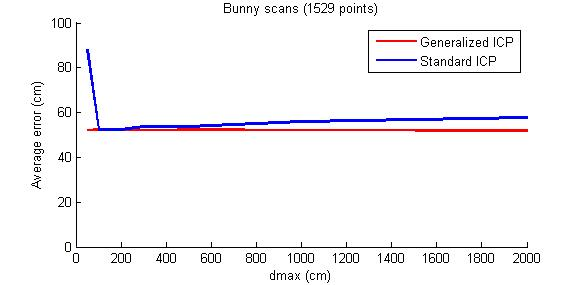
\includegraphics[scale=0.4]{Images/bunny_evol_error_dmax.jpg}
     \caption{Données synthétiques}
   \end{subfigure}%
   ~
   \begin{subfigure}[t]{.5\linewidth}
     \centering
     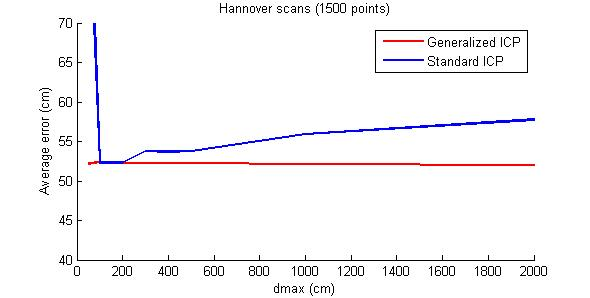
\includegraphics[scale=0.4]{Images/hannover_evol_error_dmax.jpg}
     \caption{Données réelles}
   \end{subfigure}
   
   \caption{Evolution de l'erreur de position moyenne en fonction de la valeur du seuil $d_{max}$.}
   \label{fig:err_dmax}
\end{figure}

Tout d'abord, on peut observer sur la figure \ref{fig:err_dmax} que l'influence de $d_{max}$ sur les données synthétiques est très faible.
De même, $d_{max}$ influence très peu le résultat lorsque GICP est appliqué sur les données réelles.
Au contraire, sur les données réelles qui présentent des occlusions et un recouvrement partiel, la valeur de $d_{max}$ influence fortement l'erreur pour Standard ICP 


\begin{figure}[!h]
   \centering
   \begin{subfigure}[t]{.5\linewidth}
     \centering
     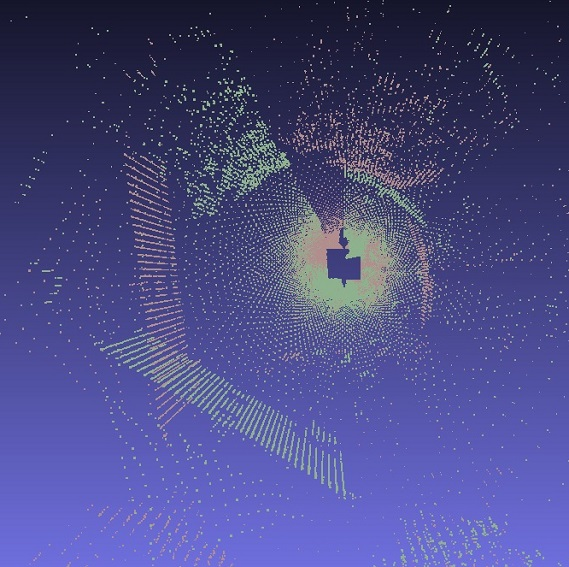
\includegraphics[scale=0.5]{Images/hannover_meshlab_before_transformation.jpg}
     \caption{Nuages avant recalage}
   \end{subfigure}%
   ~
   \begin{subfigure}[t]{.5\linewidth}
     \centering
     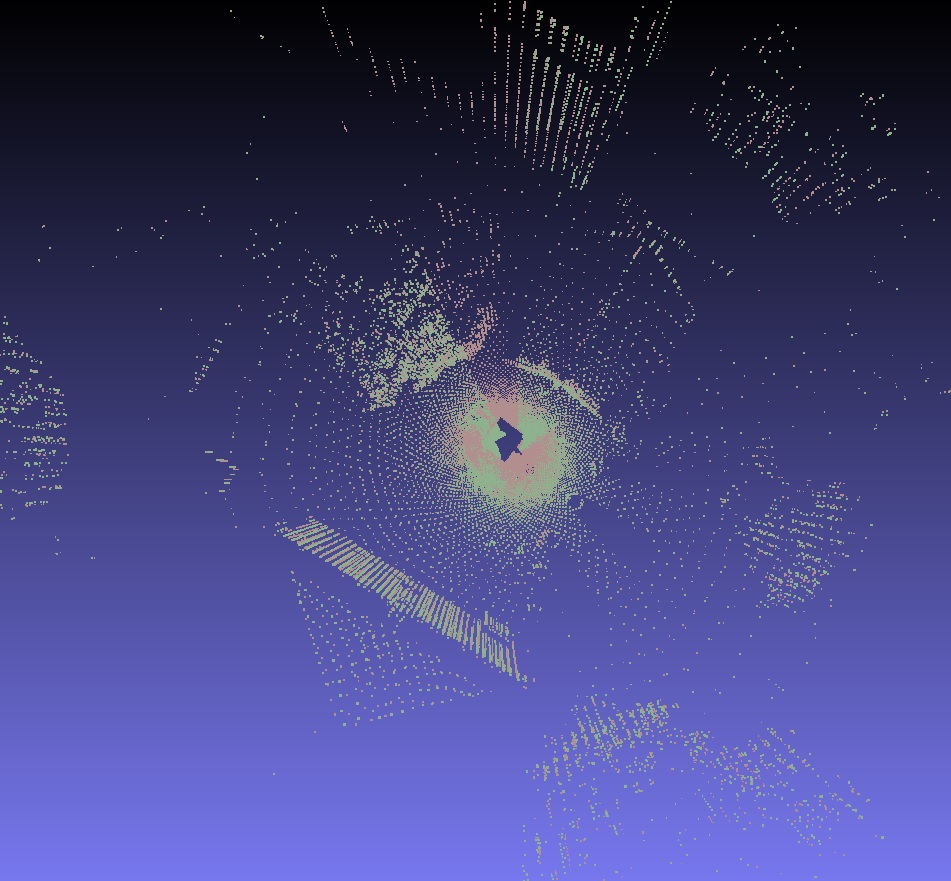
\includegraphics[scale=0.5]{Images/hannover_meshlab_after_transformation.jpg}
     \caption{Nuages après recalage}
   \end{subfigure}
   
   \caption{A REMPLIR.}
   \label{fig:meshlab}
\end{figure}
%Analyse des résultats
\subsubsection{Etude de l'influence de l'offset}


\subsubsection{Standard ICP par solution analytique}

